%================================================================================
%       Safety Critical Systems Club - Data Safety Initiative Working Group
%================================================================================
%                       DDDD    SSSS  IIIII  W   W   GGGG
%                       D   D  S        I    W   W  G   
%                       D   D   SSS     I    W W W  G  GG
%                       D   D      S    I    WW WW  G   G
%                       DDDD   SSSS   IIIII  W   W   GGG
%================================================================================
%               Data Safety Guidance Document - LaTeX Source File
%================================================================================
%
% Description:
%   Miscellanea section.
%
%================================================================================
\chapter{Lifecycle\index{Lifecycle|textbf} Considerations} \label{bkm:lifecycle}

\dsiwgSectionQuote{Failure is an amazing data point that tells you which direction not to go.}{Payal Kadakia}

\section{Usage Scenarios}
If safety-related data is incorrect it can become dangerous when used, either by making a computer or control system perform inappropriate actions, or by misleading human users into making inappropriate decisions. Since the danger can only be determined when the usage of the data is understood, risk assessment should involve both the consumer and the producer of the data.

\begin{figure}[htbp]
  \centering
  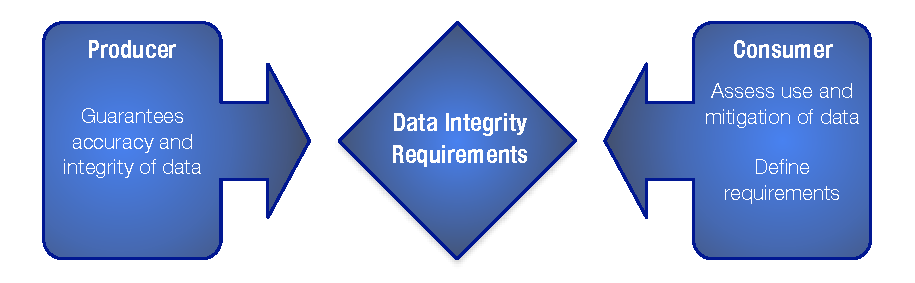
\includegraphics[width=0.75\textwidth]{images/producerconsumer}
  %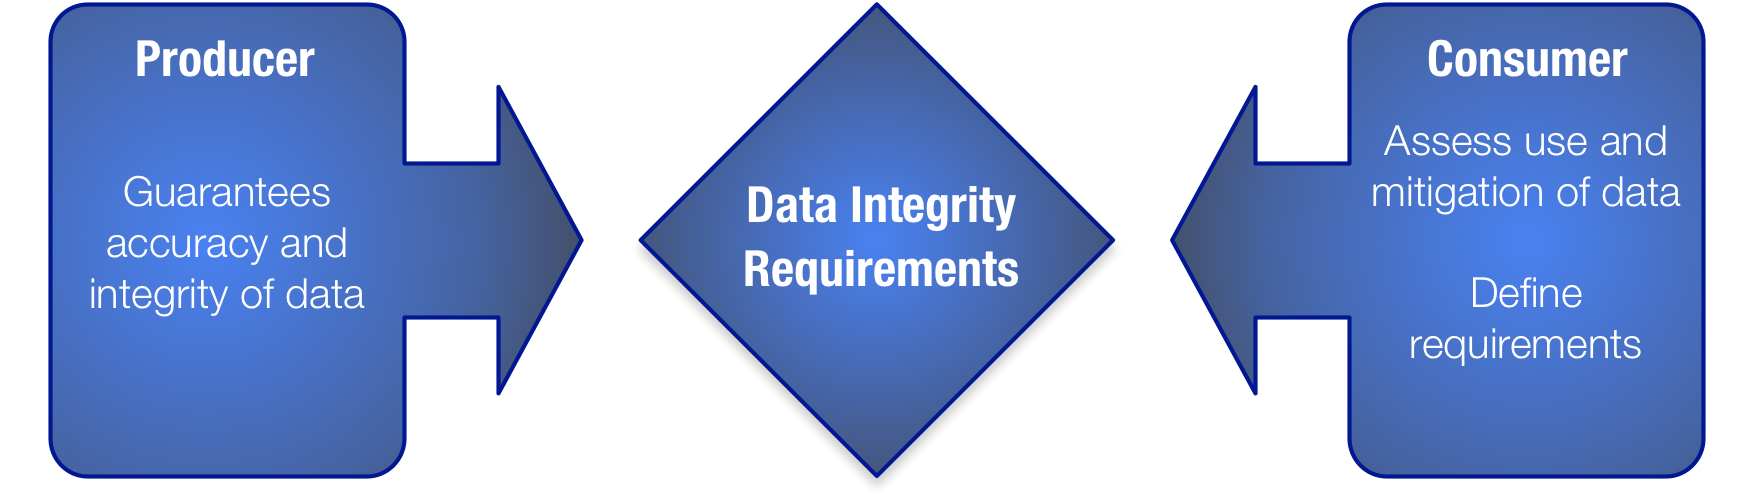
\includegraphics[width=0.75\textwidth]{images/producerconsumer.png}
  \caption{Consumer-focused \index{Integrity Property}\glsfmttext{integrity} requirements}
  \label{fig:producerconsumer}
\end{figure}

The producer investigates how the safety-related data is collected and what errors might occur. Building on activities in later phases of the data safety management process, the producer can provide some form of guarantee, or level of confidence, that the safety-related data meets the specific data-related requirements.

The consumer assesses the use of the safety-related data. In later phases of the data safety management process this \gls{information} is used to define the required \glspl{data property}: for example, how accurate a particular safety-related \index{Artefact, Data}\gls{data artefact} must be.

In some cases a producer will be providing safety-related data without any knowledge of a specific user (e.g., mapping data or generic \glspl{database} that are sold to many users). In these cases the producer will need to make some assumptions about possible users, and then clearly state what level of \index{Integrity Property}\gls{integrity} the data has been produced to. It is then up to the users to check whether the declared \index{Integrity Property}\gls{integrity} matches their need.

\section{Ways that Data Can Cause Problems}
\label{tab:issues}
\hl{???Originally said Volume 1, but it seems to fit here better.}
There are some risk-inducing issues that are different or more prevalent for data than for other system elements. An incomplete collection of examples is provided below. This list may provide a quick way of identifying risks, which could be especially useful at an early stage of a project:

\begin{description}
	\item[Fluidity:] Hardware and software can undergo significant amounts of product assurance and once assured may change relatively infrequently. Where change is required to hardware or software, it can be carefully managed and the impact on the safety case appraised. This is not always the case for data, which is often much more fluid. Indeed, the ease with which data can be changed is one motivation for the move towards \glspl{data-driven system}. This fluidity means that it is not always possible to revisit safety cases when data changes. For example, the safety case for an autonomous vehicle cannot be updated every time that the vehicle acquires new knowledge during operation. Instead, the fact that data can change, along with any associated safety impacts, may need to be captured in the system safety case. Fluidity can also provide a temptation for unscrupulous operators to falsify data, for example, after an incident has occurred. Rigorous configuration control procedures can help protect against this type of behaviour.
	
	\item[Reuse:] For the purposes of this discussion, ``reuse'' is interpreted as use of the same data in a different system or system context (e.g., lifecycle\index{Lifecycle!System} phase). Just because data was valid for use in a particular system, it does not immediately follow that it can be reused again in a similar system. Many considerations associated with data reuse are similar to those of software reuse, for example, similarity of requirements, similarity of role in the system, and similarity of required \index{Integrity!Property}\gls{integrity} / \index{Assurance Level}assurance level. One consideration that is different is that of \gls{timeliness}\index{Timeliness Property}: data that was valid for use in a particular system at a particular time is not necessarily valid for reuse in the same system at a different time.
	
	\item[Ageing:] As highlighted above, all safety-related data has a lifetime\index{Lifetime Property} and this needs to be explicitly managed. This can involve, for example, purging, deleting and alerting. Ageing can occur as a result of changes external to the system (for example, records of the positions of other aircraft, newly discovered drug interactions, or new software patches), or it can result from internal changes (e.g., valves gradually becoming less responsive, \gls{configuration data} becoming out of date, or data schemas evolving over time).
	
	\item[Transformation:] Data is often filtered, mapped or aggregated as it moves through systems, sometimes creating new \glspl{dataset} as a result. \Glspl{data property} are not necessarily preserved by these processes. Sometimes data is filtered too much or only some of the data is selected (either deliberately or inadvertently through accident or unintended bias), such as by the selection of only the test runs that succeeded. The main issues are loss of heritage / history / source \gls{information}. Data can also appear to become something else. Without careful management, the \index{Integrity!Property}\gls{integrity} may become lowered to the lowest common denominator and this needs to be recognized. Additional checks (e.g., \gls{validation} checks, credibility checks) or assurance measures may be needed to ensure that required \index{Integrity!Property}\gls{integrity} / assurance is maintained.
	
	\item[Archiving and retrieval:] Safety-related data needs to be available when required. Data \gls{accessibility}\index{Accessibility Property} needs to be considered over the complete system lifetime. It is also important to consider what \index{Data Property}properties of the data need to be preserved and how this affects the choice of storage medium.
	
	\item[Biasing:] This is a systemic inaccuracy in data due to the characteristics of the process employed in the creation, collection, manipulation, presentation, and interpretation of data. It is usually an unintentional distortion in the \gls{dataset}. One example of this is the confirmation bias that may be applied to safety claims, and another example is that synthetic autonomous vehicle training\index{Training!AI} \glspl{database} can have issues with artificial data if it is not realistic.
	Although there is no perfect way of checking for this within the system, \index{Completeness!Checks}\gls{completeness}, statistical and validity checks on \glspl{dataset} may help.
	
	\item[Falsification / misinformation:] This issue arises where data is created, modified, or deleted either accidentally or deliberately to mislead or misinform potential consumers of that data. Examples from policing and criminal justice might include notes being taken with fabricated times or dates or a crime from the wrong individual in a \gls{database} being accidentally added or removed. Another example might be a supplier falsifying quality records for materials or goods. There have been many cases of misinformation related to the Covid-19\index{Covid-19} pandemic (for example on social media) where people have been deliberately misled, and sometimes this has led to harm (for example, bleach being drunk as a cure). Possible \glspl{mitigation}\index{Mitigation} include digitally signing transmitted data, strong access controls, independent fact-checking, and audit records.
	
	\item[Defaulting:] Many systems use default or initial values for \glspl{item data}; sometimes in \glspl{dataset} and sometimes embedded in software. Often these default values are designed to be neutral (e.g., ``0'') or unrealistic (e.g., ``VOID''). There are essentially two cases:
	\begin{enumerate}
		\item initialisation data which may persist and be mistakenly taken as a real value when in fact it should have been changed; and
		\item data that is used when no meaningful value has been assigned (e.g., during data migration or data exchange between systems).
	\end{enumerate}	
	These issues can often be managed through good design of data structures, for example by the inclusion of a validity flag.
	
	\item[Sentinels:] A sentinel value is a data value that is used to indicate a special action needs to be taken, typically indicating the end of a record or a \gls{dataset}. The sentinel value should be one that is not allowable in the \gls{dataset} itself but often is not properly considered and may use common sequences (e.g., five zeroes). Sentinels can cause problems in two ways:
	\begin{enumerate}
		\item where they are not recognized and so, for example, processing includes or continues past the sentinel; and
		\item where the data itself somehow contains the sentinel value and so processing is erroneously interrupted.
	\end{enumerate}
	Sentinels can be a particular risk in long-lived systems and \glspl{dataset}. As with defaulting, the management or elimination of this issue may often be achieved through improved data structures.
	
	\item[Aliasing:] This is an effect that causes different data to become indistinguishable when accessed; that is, there is only one record when there should be several -- for example, two patients with similar names inadvertently sharing a single set of medical records. This could be due to the way the data is filtered, sampled, indexed, stored, or retrieved. The data issues are typically related to loss of resolution leading to similar data points appearing to be identical. Methods to maintain resolution, including use of unique indexes, may be beneficial.
	
	One specific case of aliasing  concerns homophones -- words which sound the same but are different such as ``flower'' / ``flour'' and ``bare'' / ``bear'' \cite{citation:homonym}.
	If these words are read out over a phone there may be confusion as to which is intended.
	Location services based on a number of words such as W3W don't avoid all homophones,
	and so there may be issues when the words are given verbally in an emergency. The issue is discussed further in Section \autoref{bkm:incacc:w3w}.
	
	\item[Disassociation:] This effect is, in some senses, the opposite of aliasing: there are several records when there should only be one. This could occur, for example, if two records are created for the same individual using slightly different names. It could also arise if different systems use different indexing methods and the association between the indexes becomes corrupted. Again, methods to maintain data resolution can be beneficial.
	
	\item[Masking:] This issue can arise if a notable proportion of a \gls{dataset} is of a poor \gls{quality}, for example, if sensors producing the data are faulty or measurements are taken from the wrong source. This poor quality data can mask errors in the way that the system handles the good quality data. One way of protecting against this issue is the generation and use of test sets of appropriate size and quality, although for some applications this may be a non-trivial task.
	
	\item[Incompleteness:]\index{Completeness!Property} Not all the data that is needed is always available; there may be known, and sometimes, unknown gaps or missing data points. The missing data points (``dark data''\index{Dark Data} -- see Section \dsiwgExtRef{Section}{2}{bkm:darkdata}) can be critical and in some cases, more important than the data that is available. Incomplete data can arise, for example, from limitations on how much data can be physically captured (e.g. sampling frequencies, storage / time constraints) or from the unintentional or deliberate darkening of data (e.g. for privacy, security, political or commercial reasons).
	
	\item[Volume:] Data can be so large and unstructured that it is not manageable in practicable timeframes.
	For example, video records of rail track could take days to inspect manually.
	
	\item[Interpretation:] Data can be misinterpreted -- too much or too little deduced from available data, or data extrapolated incorrectly to derive unsound results.
	An example is \gls{ml} data\index{Machine Learning Data}, especially real or recorded data that may not contain critical edge / corner cases.
	
	\item[Distribution:] Data can be decentralised, decomposed or distributed across many sources (e.g. channels, \glspl{database}, websites) and needs to be consistently integrated to make a coherent picture. In the health sector many IT systems often have to work together feeding in different parts of a patient medical record to make a complete health picture. If parts of this distributed data are missing (for instance diagnostic test results) then it is difficult if not impossible to obtain the complete picture, and mistakes may be made.
	There are several parts to this problem:
	\begin{description}
		\item[Integration] -- multiple elements of data have to be brought together in a coherent way, addressing aspects such as which data should supercede or replace other data;
		\item[Communication] -- having correct and current \gls{information} about what data is available and its location so it can be requested; and
		\item[Contingency:] -- what to to if part of the distributed data is unavailable or late.
	\end{description}
\end{description}


Further examples of how data may cause issues in many scenarios is given in the book \dsiwgTextIT{Data-Centric Safety: Challenges, Approaches, and Incident Investigation} \cite{citation:datacentric}.

\section{\ecapitalisewords{\glsentryplural{data property}}}\label{bkm:guidance:dataproperties}
\hl{???Originally said move to Volume 1, but I think it fits better here.}
\Glspl{data property} are used to establish what aspects of the data (e.g., \gls{timeliness}\index{Timeliness Property}, \gls{accuracy}\index{Accuracy Property}) need to be guaranteed in order that the system operates in a safe manner.

James Inge's work \cite{citation:inge2008improving} produced a useful taxonomy of data categories, and went on to look at faults in data. He concluded that a rigid taxonomy of data categories was unhelpful due to various properties or characteristics of the data which vary independently. In short, it is the combination of data category\index{Category!Data} with the required \index{Data Property}\glspl{data property} that facilitates safety analysis.

Data categories were discussed \dsiwgExtRef{Chapter}{2}{Part2-bkm:categories}. \autoref{tab:PropertiesOfData} documents a non-exhaustive collection of \index{Data Property}\glspl{data property}. Typically, it is the loss of one of these \glspl{data property} that presents a \gls{hazard}. This notion of ``loss'' is dependent on the intended use; for example, what is ``timely'' for one use may not be for another.

The ``\Gls{goldilocks}''\index{Goldilocks Property} property\footnote{The authors are aware that some of the names of categories are very culturally dependent. For example, we are informed that the folk-tale of Goldilocks is not well known in Chinese culture but the idiom gu\`oy\'oub\`uj\'\i, interpreted as ``doing too much is just as bad as not doing enough'' is well known. The intention of the names is simply to evoke the associations, so users of this guidance are encouraged to use names for the categories that are more appropriate to their cultures.} addresses appropriate sizing and quantity of data. A number of issues have been found to arise when there is too much or too little data. While it is particularly relevant to communications links, it may have relevance to other areas such as \glspl{database} and when people are involved in reviewing or checking data. The property is named ``\gls{goldilocks}'' as it refers to the need to have not too much, not too little, but just the right amount of data%
%
\hl{??? LaTeX crashes if I have this footnote on the same page as a longtable.}
A system where the property was lost involved a high-speed data bus that connected several safety-critical systems. A transceiver of that bus failed and transmitted random noise. The receivers employed parity checks and cyclic redundancy check, but the system had been designed to eliminate occasional \glspl{error}. When random noise filled the bus, several apparently valid messages were created every second, resulting in potentially lethal behaviour.
	
	In a \gls{hazop}\index{HAZOP} carried out during 2020, based upon the \gls{hazop}\index{HAZOP} guidewords in this guidance, the facilitator realised that certain failure modes had not been identified by the \gls{hazop} team. In addition to the issue of system overload already discussed, those omissions also concerned system behaviour following data rejection. In these cases, bad data was detected and rejected, but the consequences of data rejection over an extended period had not been considered.

The \gls{goldilocks}\index{Goldilocks Property} property is related to the data volume problem discussed in \hyperref[tab:issues]{section}~\ref{tab:issues}, however, given the importance of data sizing and the experience of real-world incidents this is now a separate property.

%
\subsection{The \glsfmttext{analysability}\index{Analysability Property} property}\label{bkm:guidance:analysability}
The \gls{analysability} property recognizes that data is now highly complex and extensive, often large scale, and distributed. And yet, for safety purposes we need to make sure it is of suitable quality and able to support system goals.
We therefore need to ensure that it is possible to analyse it for key characteristics and establish meaningful results using tools or other means. This property is related to explainabilty and may be performed by the same set of tools or techniques.

\subsection{The \glsfmttext{explainability}\index{Explainability Property} property}\label{bkm:guidance:explainability}
\Gls{explainability} describes the ability to establish what the purpose and effect data (and especially changes to data) has on a system
and explain this to relevant \glspl{stakeholder} in terms that they can understand. It is particularly important for learning and AI-based systems.
This could be, for example, \gls{ml} training\index{Training!AI} data or system \gls{configuration data}.
This property is related to \gls{analysability}\index{Analysability Property} and may be performed by the same set of tools or techniques.
%
\begin{longtable}{|L{\dsiwgColumnWidth{0.24}}|C{\dsiwgColumnWidth{0.15}}|L{\dsiwgColumnWidth{0.61}}|}
	\caption{\index{Data Property}Properties of data}
	\label{tab:PropertiesOfData}
	\\\hline\TableHeadColour{Property} & \TableHeadColour{Abbreviation} & \TableHeadColour{Description}\\\hline
	\endfirsthead
	\caption[]{Properties of data (continued)}
	\\\hline\TableHeadColour{Property} & \TableHeadColour{Abbreviation} & \TableHeadColour{Description}\\\hline
	\endhead
	\multicolumn{3}{r}{\sl Continued on next page}
	\endfoot
	\endlastfoot
	\Gls{integrity}\index{Data Property!Integrity|see {Integrity, Property}}\index{Integrity!Property} & I & The data is correct, true and unaltered\\\hline
	\Gls{completeness}\index{Data Property!Completeness|see {Completeness, Property}}\index{Completeness!Property} & C & The data has nothing missing or lost\\\hline
	\Gls{consistency}\index{Data Property!Consistency|see {Consistency Property}}\index{Consistency!Property} & N & The data adheres to a common world view (e.g., units)\\\hline
	{\Gls{continuity}}\index{Data Property!Continuity|see {Continuity Property}}\index{Continuity Property} & Y & {The data is continuous and regular without gaps or breaks}\\\hline
	{\Gls{format}}\index{Data Property!Format|see {Format Property}}\index{Format Property} & O & {The data is represented in a way which is readable by those that need to use it}\\\hline
	{\Gls{accuracy}}\index{Data Property!Accuracy|see {Accuracy Property}}\index{Accuracy Property} & A & {The data has sufficient detail for its intended use}\\\hline
	{\Gls{resolution}}\index{Data Property!Resolution|see {Resolution Property}}\index{Resolution Property} & R & {The smallest difference between two adjacent values that can be represented in a data storage, display or transfer system}\\\hline
	{\Gls{traceability}}\index{Data Property!Traceability|see {Traceability Property}}\index{Traceability Property} & T & {The data can be linked back to its source or derivation}\\\hline
	{\Gls{timeliness}}\index{Data Property!Timeliness|see {Timeliness Property}}\index{Timeliness Property} & M & {The data is as up to date as required}\\\hline
	{\Gls{verifiability}}\index{Data Property!Verifiability|see {Verifiability Property}}\index{Verifiability Property} & V & {The data can be checked and its properties demonstrated to be correct}\\\hline
	{\Gls{availability}}\index{Data Property!Availability|see {Availability Property}}\index{Availability Property} & L & {The data is accessible and usable when an authorized entity demands access}\\\hline
	{\Gls{fidelity}}\index{Data Property!Fidelity|see {Fidelity Property}}\index{Fidelity Property} & F & {How well the data maps to the real-world entity it is trying to model}\\\hline
	{\Gls{priority}}\index{Data Property!Priority|see {Priority Property}}\index{Priority Property} & P & {The data is presented / transmitted / made available in the order required}\\\hline
	{\Gls{sequencing}}\index{Data Property!Sequencing|see {Sequencing Property}}\index{Sequencing Property} & Q & {The data is preserved in the order required}\\\hline
	{\Gls{intended_destination}}\index{Data Property!Intended Destination|see {Intended Destination Property}}\index{Intended Destination Property} & U & {The data is only sent to those that should have access to it}\\\hline
	{\Gls{accessibility}}\index{Data Property!Accessibility|see {Accessibility Property}}\index{Accessibility Property} & B & {The data is visible only to those that should see it}\\\hline
	{\Gls{suppression}}\index{Data Property!Suppression|see {Suppression Property}}\index{Suppression Property} & S & {The data is intended never to be used again}\\\hline
	{\Gls{history}}\index{Data Property!History|see {History Property}}\index{History Property} & H & {The data has an audit trail of changes}\\\hline
	{\Gls{lifetime}}\index{Data Property!Lifetime|see {Lifetime Property}}\index{Lifetime Property} & E & {When does the safety-related data expire}\\\hline
	{\Gls{disposability}}\index{Data Property!Disposability|see {Disposability Property}}\index{Disposability Property} & D & {The data can be permanently removed when required}\\\hline
	{\Gls{goldilocks}}\index{Data Property!Goldilocks|see {Goldilocks Property}}\index{Goldilocks Property} & G & {The data is just the right size -- not too much and not too little}\\\hline
	{\Gls{analysability}}\index{Data Property!Analysability|see {Analysability Property}}\index{Analysability Property} & Z & {The data (including any \gls{metadata}) is of a suitable size, type and format to enable it be usefully analysed}\\\hline
	{\Gls{explainability}}\index{Data Property!Explainability|see {Explainability Property}}\index{Explainability Property} & X & {The data can be meaningfully explained,by a suitable mechanism, to those who need to understand it}\\\hline
	{\Gls{clarity}}\index{Data Property!Clarity|see {Clarity Property}}\index{Clarity Property} & K & {The data is visible, unmasked, not hidden or obscured and not camouflaged}\\\hline
\end{longtable}

\autoref{tab:issuesCrossReference} illustrates where the data issues discussed in
\hyperref[tab:issues]{Section}~\ref{tab:issues} %Clunky, but \autoref inserted "subsubsection"
can result in
loss of one or more \index{Data Property}data properties (x = potential loss of property).

\begin{longtable}{|L{\dsiwgColumnWidth{0.15}}|%
		C{\dsiwgColumnWidth{0.034}}|C{\dsiwgColumnWidth{0.034}}|C{\dsiwgColumnWidth{0.034}}|C{\dsiwgColumnWidth{0.034}}|%
		C{\dsiwgColumnWidth{0.034}}|C{\dsiwgColumnWidth{0.034}}|C{\dsiwgColumnWidth{0.034}}|C{\dsiwgColumnWidth{0.034}}|%
		C{\dsiwgColumnWidth{0.034}}|C{\dsiwgColumnWidth{0.034}}|C{\dsiwgColumnWidth{0.034}}|C{\dsiwgColumnWidth{0.034}}|%
		C{\dsiwgColumnWidth{0.034}}|C{\dsiwgColumnWidth{0.034}}|C{\dsiwgColumnWidth{0.034}}|C{\dsiwgColumnWidth{0.034}}|%
		C{\dsiwgColumnWidth{0.034}}|C{\dsiwgColumnWidth{0.034}}|C{\dsiwgColumnWidth{0.034}}|C{\dsiwgColumnWidth{0.034}}|%
		C{\dsiwgColumnWidth{0.034}}|C{\dsiwgColumnWidth{0.034}}|C{\dsiwgColumnWidth{0.034}}|C{\dsiwgColumnWidth{0.034}}|}
	\caption{Properties that can be lost through issues}
	\label{tab:issuesCrossReference}
	\\\hline
	& \rotatebox{90}{\index{Integrity!Property}\Gls{integrity}}
	& \rotatebox{90}{\index{Completeness!Property}\Gls{completeness}}
	& \rotatebox{90}{\index{Consistency!Property}\Gls{consistency}}
	& \rotatebox{90}{\index{Continuity Property}\Gls{continuity}}
	& \rotatebox{90}{\index{Format Property}\Gls{format}}
	& \rotatebox{90}{\index{Accuracy Property}\Gls{accuracy}}
	& \rotatebox{90}{\index{Resolution Property}\Gls{resolution}}
	& \rotatebox{90}{\index{Traceability Property}\Gls{traceability}}
	& \rotatebox{90}{\index{Timeliness Property}\Gls{timeliness}}
	& \rotatebox{90}{\index{Verifiability Property}\Gls{verifiability}}
	& \rotatebox{90}{\index{Availability Property}\Gls{availability}}
	& \rotatebox{90}{\index{Fidelity Property}\Gls{fidelity}}
	& \rotatebox{90}{\index{Priority Property}\Gls{priority}} 
	& \rotatebox{90}{\index{Sequencing Property}\Gls{sequencing}}
	& \rotatebox{90}{\index{Intended Destination Property}\Gls{intended_destination}}
	& \rotatebox{90}{\index{Accessibility Property}\Gls{accessibility}}
	& \rotatebox{90}{\index{Suppression Property}\Gls{suppression}}
	& \rotatebox{90}{\index{History Property}\Gls{history}}
	& \rotatebox{90}{\index{Lifetime Property}\Gls{lifetime}}
	& \rotatebox{90}{\index{Disposability Property}\Gls{disposability}}
	& \rotatebox{90}{\index{Goldilocks Property}\Gls{goldilocks}}
	& \rotatebox{90}{\index{Analysability Property}\Gls{analysability}}
	& \rotatebox{90}{\index{Explainability Property}\Gls{explainability}}
	& \rotatebox{90}{\index{Clarity Property}\Gls{clarity}}
	%
	\\\hline\TableHeadColour{Issue} &%
	\TableHeadColour{I} & \TableHeadColour{C} & \TableHeadColour{N} & \TableHeadColour{Y} &%
	\TableHeadColour{O} & \TableHeadColour{A} & \TableHeadColour{R} & \TableHeadColour{T} &%
	\TableHeadColour{M} & \TableHeadColour{V} & \TableHeadColour{L} & \TableHeadColour{F} &%
	\TableHeadColour{P} & \TableHeadColour{Q} & \TableHeadColour{U} & \TableHeadColour{B} &%
	\TableHeadColour{S} & \TableHeadColour{H} & \TableHeadColour{E} & \TableHeadColour{D} &%
	\TableHeadColour{G} & \TableHeadColour{Z} & \TableHeadColour{X} & \TableHeadColour{K} \\\hline
	\endfirsthead
	\caption[]{Properties that can be lost through issues (continued)}
	\\\hline
	& \rotatebox{90}{\index{Integrity!Property}\Gls{integrity}}
	& \rotatebox{90}{\index{Completeness!Property}\Gls{completeness}}
	& \rotatebox{90}{\index{Consistency!Property}\Gls{consistency}}
	& \rotatebox{90}{\index{Continuity Property}\Gls{continuity}}
	& \rotatebox{90}{\index{Format Property}\Gls{format}}
	& \rotatebox{90}{\index{Accuracy Property}\Gls{accuracy}}
	& \rotatebox{90}{\index{Resolution Property}\Gls{resolution}}
	& \rotatebox{90}{\index{Traceability Property}\Gls{traceability}}
	& \rotatebox{90}{\index{Timeliness Property}\Gls{timeliness}}
	& \rotatebox{90}{\index{Verifiability Property}\Gls{verifiability}}
	& \rotatebox{90}{\index{Availability Property}\Gls{availability}}
	& \rotatebox{90}{\index{Fidelity Property}\Gls{fidelity}}
	& \rotatebox{90}{\index{Priority Property}\Gls{priority}} 
	& \rotatebox{90}{\index{Sequencing Property}\Gls{sequencing}}
	& \rotatebox{90}{\index{Intended Destination Property}\Gls{intended_destination}}
	& \rotatebox{90}{\index{Accessibility Property}\Gls{accessibility}}
	& \rotatebox{90}{\index{Suppression Property}\Gls{suppression}}
	& \rotatebox{90}{\index{History Property}\Gls{history}}
	& \rotatebox{90}{\index{Lifetime Property}\Gls{lifetime}}
	& \rotatebox{90}{\index{Disposability Property}\Gls{disposability}}
	& \rotatebox{90}{\index{Goldilocks Property}\Gls{goldilocks}}
	& \rotatebox{90}{\index{Analysability Property}\Gls{analysability}}
	& \rotatebox{90}{\index{Explainability Property}\Gls{explainability}}
	& \rotatebox{90}{\index{Clarity Property}\Gls{clarity}}
	%
	\\\hline\TableHeadColour{Issue} &%
	\TableHeadColour{I} & \TableHeadColour{C} & \TableHeadColour{N} & \TableHeadColour{Y} &%
	\TableHeadColour{O} & \TableHeadColour{A} & \TableHeadColour{R} & \TableHeadColour{T} &%
	\TableHeadColour{M} & \TableHeadColour{V} & \TableHeadColour{L} & \TableHeadColour{F} &%
	\TableHeadColour{P} & \TableHeadColour{Q} & \TableHeadColour{U} & \TableHeadColour{B} &%
	\TableHeadColour{S} & \TableHeadColour{H} & \TableHeadColour{E} & \TableHeadColour{D} &%
	\TableHeadColour{G} & \TableHeadColour{Z} & \TableHeadColour{X} & \TableHeadColour{K}\\\hline
	\endhead
	\multicolumn{22}{r}{\sl Continued on next page}
	\endfoot
	\endlastfoot
	Fluidity       &   &   &   &   &   &   &   & x &   & x &   & x &   &   &   &   &   & x &   &   & x & x & x & x \\\hline
	Reuse          &   & x &   &   &   & x &   & x & x & x &   & x &   &   & x &   & x & x & x & x & x &   & x & \\\hline
	Ageing         &   & x &   &   &   & x &   &   & x &   &   & x &   &   & x & x & x & x & x & x & &   & x & \\\hline
	Transformation & x & x & x & x & x & x & x & x & x & x & x & x & x & x & x & x & x & x & x & x & x & x & x & x \\\hline
	\index{Data!Owner}Ownership      &   &   &   &   &   &   &   & x &   & x & x &   &   &   & x & x &   & x &   &   &   &   & x & \\\hline
	Archiving / retrieval &   &   &   &   &   &   &   &   &   &   &   &   &   &   & x & x & x & x & x & x &   & x & & x \\\hline
	Biasing        & x & x & x & x &   & x &   &   & x & x &   & x & x & x &   &   &   &   &   &   &   & x & x & \\\hline
	Falsification / misinformation & x & x & x & x & x & x & x & x & x & x & x & x & x & x & x & x & x & x & x & x & x & x & x & x \\\hline
	Defaulting     & x & x & x & x &   & x &   &   &   &   &   & x &   &   &   &   &   &   &   &   &   & x & & x \\\hline
	Sentinels      & x & x &   & x &   & x &   &   &   &   &   &   &   & x &   &   &   &   &   &   &   & x & & x \\\hline
	Aliasing       & x & x &   & x &   & x & x & x &   & x & x & x &   &   &   &   &   &   &   &   &   & x & x &  x \\\hline
	Disassociation & x &   &   & x &   & x &   & x & x & x & x & x & x & x & x & x & x & x & x & x &   & x & x & x \\\hline
	Masking        & x & x & x & x &   & x &   &   &   & x &   & x &   &   &   &   &   &   &   &   &   & x & x & x \\\hline
	\index{Completeness!Property}Incompleteness & x & x & x & x & x & x & x & x & x & x & x & x & x & x & x & x & x & x & x & x & x & x & x & x \\\hline
	Volume         &   &   &   &   &   &   &   &   &   & x &   &   &   &   &   &   &   &   &   &   & x & x & x & x \\\hline
	Interpretation & x & x & x &   & x & x & x &   & x & x &   & x &   &   &   &   &   &   &   &   &   & x & x & \\\hline
	Distribution   & x & x & x & x &   &   &   & x &   &   & x &   & x & x & x & x &   & x &   & x &   & x & x & x \\\hline
\end{longtable}
\section{Data in System Lifecycles}
Like other components of a safety-related system, the safety dependency of data is dictated by the context in which it is used and the causal links that become established where loss of one or more of the required \index{Property!Data}properties can contribute to hazardous system states. For example, a given \gls{dataset} (say \gls{configuration data}) could be used in a number of separate contexts such as:
\begin{itemize}
  \item prototyping a system to demonstrate solution feasibility of a safety-related system;
  \item development testing of a safety-related system; and
  \item live operational use of a safety-related system.
\end{itemize}

In these cases, the \gls{dataset} is the same but the context of its use changes the safety significance and therefore the level of assurance that it may require. It follows that the \gls{dsal} of a \gls{dataset} is also predicated on where and when in the lifecycle the \gls{dataset} will be applied. 

To illustrate this concept, a number of generic model lifecycles are discussed below. Note that these are not intended to be prescriptive or mandate the use of any particular model. Instead, they are being used to illustrate how the Data Safety Management Plan could articulate these lifecycle considerations.

\dsiwgTextBF{Development:} the diagram in \autoref{fig:developmentlifecycle} represents a typical development lifecycle using an iterative development approach\footnote{The diagram is based on \gls{ibm}'s Rational Unified Process, an iterative software development\index{Software Development Process} process framework. The original diagram is in the public domain.}. In this model there are key phases as the system transitions from concept through to testable executable code. The process is iterative in that several cycles of functional elaboration, design, development and test may be run and these typically will focus on the areas of the system that bear most technical risk or comprise the key functional use cases so the client gets early visibility of the system. This early awareness allows feedback to be provided into the next iteration to help steer the solution to the client's actual needs. Traditional waterfall implementation can map onto this model on the basis that there is only one iteration in each phase and all activities in one phase need to be completed before progressing to the next.

\begin{figure}[htbp]
  \centering
  %\includegraphics[width=\textwidth]{images/developmentlifecycle}
  %\includegraphics[width=\textwidth]{images/developmentlifecycle_png600}
  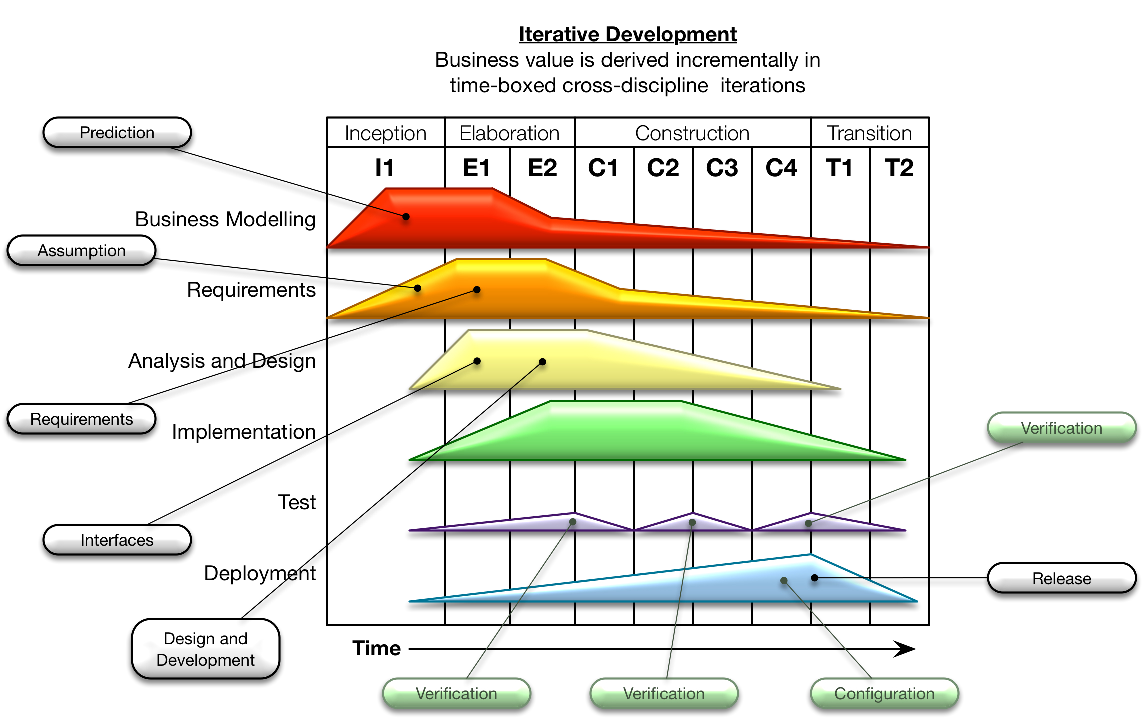
\includegraphics[width=\textwidth]{images/developmentlifecycleflat}
  \caption{Development lifecycle}
  \label{fig:developmentlifecycle}
\end{figure}

The model itself may vary depending on the specific needs of the project but the diagram illustrates that different data categories\index{Category!Data} become significant at different points of the process. 

\dsiwgTextBF{Operational} Once a system has been developed it will move into an operational lifecycle or indeed, if data safety has not previously been considered for an enterprise, then the system could already be in operational use. These operational lifecycles tend to be cyclical in nature; the diagram in \autoref{fig:operationallifecycle}\footnote{ITIL is a registered Trade Mark of AXELOS Limited. All rights reserved.} illustrates a typical model.

\begin{figure}[htbp]
  \centering
  %\includegraphics[width=0.9\textwidth]{images/operationallifecycle}
  %\includegraphics[width=0.9\textwidth]{images/operationallifecycle_png600}
  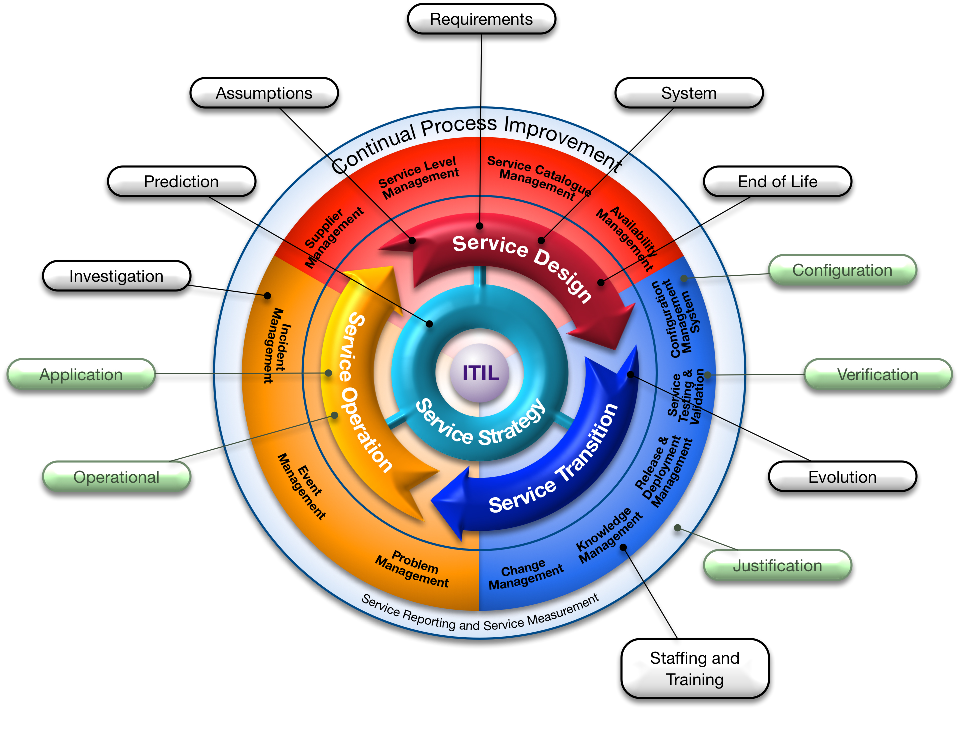
\includegraphics[width=0.9\textwidth]{images/operationallifecycleflat}
  \caption{Operational lifecycle}
  \label{fig:operationallifecycle}
\end{figure}

Again, specific data \index{Category!Data} will come into play at different periods in the process. Documenting the relationship between process steps and data categories will therefore give clarity as to when a particular assurance technique needs to be applied.

\dsiwgTextBF{Data supply chains} The previous models relate to typical system supply and operate perspectives but there are also other data supply chains where a number of organizations engage in the procurement and use of safety-related data. These processes may include the development and operational lifecycles but a different model is required to fully represent the wider processes that are being employed. The diagram in \autoref{fig:dataacquisitionlifecycle} shows such a model representing a data acquisition lifecycle.

\begin{figure}[htbp]
  \centering
  %\includegraphics[width=\textwidth]{images/dataacquisitionlifecycle}
  %\includegraphics[width=\textwidth]{images/dataacquisitionlifecycle_png600}
  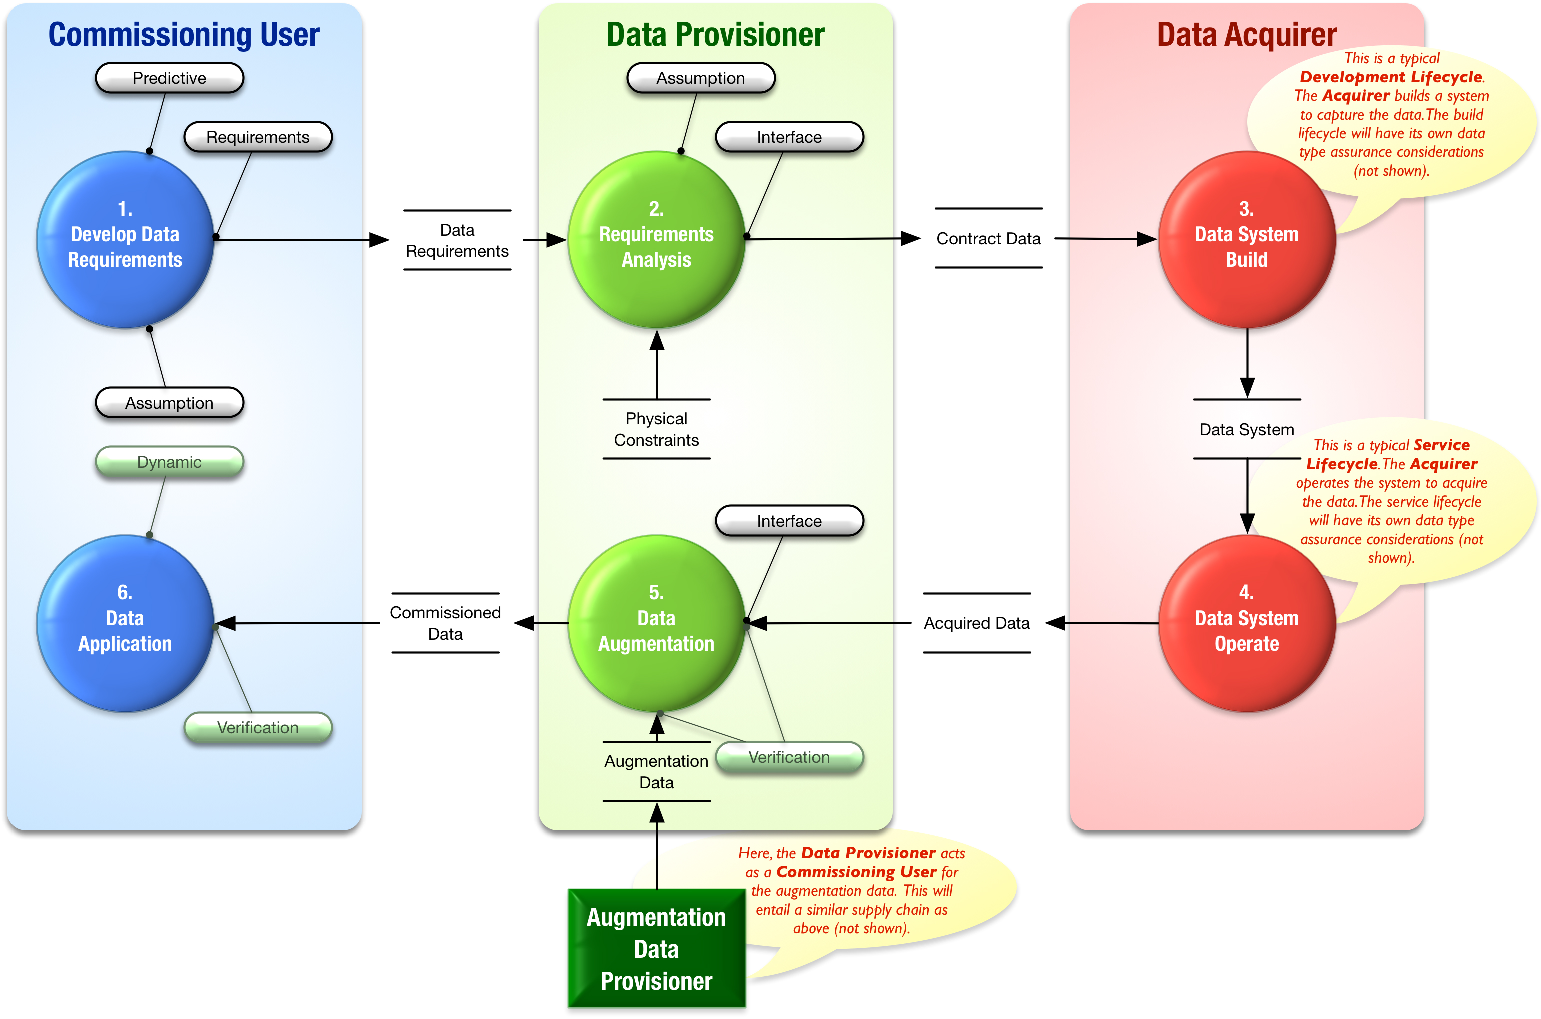
\includegraphics[width=\textwidth]{images/dataacquisitionlifecycleflat}
  \caption{Data supply chain}
  \label{fig:dataacquisitionlifecycle}
\end{figure}

This model represents the interactions between three key organizations:
\begin{itemize}
  \item The commissioning user: the organization that has the need for the data;
  \item The data provisioner: the organization that will fulfil that need for data; and
  \item The data acquirer: the organization employed by the Data Provisioner to carry out physical collection of data.
\end{itemize}

Note that these may be three separate organizations, or they may be separate business units within the same, larger, organization.

In this supply chain, the commissioning user is a consumer of the data and the data acquirer is a producer of data. The data provisioner acts both as a consumer (from the data acquirer) and producer (to the commissioning user) of data. Similarly, an organization that augments \glspl{dataset} is both a consumer and producer of data in the supply chain.

The commissioning user requirement analysis is the key process step where the commissioning user's expectations for data are agreed with the data provisioner. The requirements may be adjusted because of physical constraints (e.g., loss of precision because of physical measuring device constraints) and may include additional requirements to augment the captured data with additional \gls{information} (e.g., airport codes added to a measurement of a given runway length).

The data provisioner may employ a data acquirer to capture the data (e.g., to carry out a physical survey of a site). The acquisition phase may itself require a specialised system to be built to perform the capture and data refinement to meet the data provisioner's specifications. Such systems will then themselves be subject to the development lifecycle model considerations discussed above. Likewise, the data augmentation phase may require further system development processes or indeed, could trigger an instance of the model again as the data provisioner acting as a Commissioning User.

Acquired and augmented data is then fed into the operational system that has been built for providing the service of generating the commissioned data. This system in its service provision role would then typically follow the operational lifecycle process model discussed earlier.

\subsection{Tool Assurance}
Tools in this context are considered anything that automates all or part of a process, for example, data creation or data transformation. Test tools are also included (i.e., the term is not limited to parts of an operational system).

Tools can impact data safety in different ways, depending on both their function and how they are to be used. For tools to be considered fit for purpose it is necessary to show that the tool meets its requirements in the context in which it is to be used. The activity to ensure a tool is fit for purpose is usually called ``tool qualification''.

The first step is to define the purpose for which the tool is required to be fit. Once that is done, and the tool's requirements are specified, there are three main strategies available for qualification:
\begin{itemize}
  \item Use evidence of a previous certification of the tool by a trusted third party (unlikely to be available in most industry sectors);
  \item Base tool qualification on the practices used when designing and developing the tool (only practicable for tools developed within the organization); and
  \item Use one of the available industry-specific guidance documents that admit \gls{cots} solutions, e.g., EUROCAE Document ED-215 (RTCA/DO-330) \cite{citation:ED215}.
\end{itemize}

%There is an alternative, risk-based and perhaps more feasible, approach. This involves assessing the potential risks presented by use of the tool and providing assurance that these risks are adequately managed. The method proceeds as follows:

%\begin{itemize}
%  \item Draft a procedure for the use of the tool to achieve the stated purpose;
%  \item Identify threats to data safety associated with using the tool;
%  \item Specify adequate mitigations\index{Mitigation} for each identified threat;
%  \item Augment and formally issue the tool requirements and the usage procedure to implement the specified  mitigations\index{Mitigation%};
%  \item Demonstrate that the tool and its mitigations\index{Mitigation} perform as expected; and
%  \item Provide a compelling assurance argument based on the previous steps and any other evidence that will improve confidence; for example:
%  \begin{itemize}
%    \item reputation of the supplier; 
%    \item configuration management of the tool, its settings and its documentation;
%    \item competence of the tool user; and
%    \item checks that are made on the tool's output.
%   \end{itemize}
%\end{itemize}

Further details on tool qualification are presented in Part 2 Chapter~\ref*{Part2-bkm:tools}.

\subsection{Test Data}
The generation of suitable test data is critical to verification of a safety system. The test data must include both representative ``normal'' values based on intended usage and also values which push at, and beyond, normal use to provoke \glspl{hazard} that the system might produce. This latter type of test data is particularly hard to generate; generally it must be credible, yet it must stress the system to react in a way that the preservation of \index{Property!Safety}safety properties can be assessed. 

In general, all the \index{Property!Data}properties of the test data should be considered and an assessment made as to whether breaking a property (e.g., introducing corrupt or late data) would cause a problem to the system. If it does, then specific test data should be produced to facilitate testing of this potential problem.

Some suggestions for test data for safety-related systems are:
\begin{itemize}
  \item Use of values on or around boundaries;
  \item Use of extreme values, way beyond what could be reasonably expected;
  \item Use of typical ``everyday'' values / sets;
  \item Some realistic but unexpected values;
  \item Try combinations of data values or \glspl{item data} that are problematic together (e.g., inconsistent);
  \item If possible, use some values known to have caused problems in the past;
  \item Where appropriate, use values related to timing, rollover or date boundaries;
  \item Where possible, use white box values (i.e., those derived from an understanding of the system);
  \item Use a set of values with drift or bias over time;
  \item Use \glspl{dataset} with particular \index{Property!Statistical}statistical properties (e.g., distribution, patterns etc.);
  \item Use data which has incorrect formatting, ordering, or out of sequence, etc.; and
  \item Try data which has repeated sets of values or pseudo-random characteristics.
\end{itemize}
Typically very complex test data is derived from recorded live feeds of real data flows. While this data can be extremely useful for regression purposes, it should be recognised that it is unlikely to contain many outlying or boundary \glspl{item data}. Therefore it may need to be modified to test any hazardous situations; this modification can be difficult and may require sophisticated tools to both ensure correct \index{Property!Data}properties and injection of the intended faults (for instance to introduce a statistical bias to the data).

Simulator / emulator derived values can be useful, but again the issue is how realistic the values are: often the \index{Accuracy Property}\gls{accuracy}, \gls{resolution} or timing of simulated values may be different to real data.

Coverage with test data is something to consider. Sometimes the same \gls{dataset} is used for multiple test scenarios, when in fact it is not stressing all of them to the same degree. Test data coverage can be collected over requirements, code or design, but it is important not to forget hazards: coverage of the hazards and mitigations\index{Mitigation} identified in the \gls{hazard log} is a key aim. 

In general some measure of the quality and suitability of the test data can be useful. This could be based on \index{Property!Statistical}statistical properties, coverage of hazards or coverage of requirements. 

Test data must show continued relevance, through systems evolution\index{Evolution!System} and over time. It is good practice to build up extensive regression suites containing coverage of all detected problems to date.

\subsection{Interfaces with Existing Assessments}\index{Interface!Assessment}
\subsubsection{Data and Software}\index{Software vs. Data}
Although most people feel they have an intuitive understanding of the difference between software and data, upon closer examination the boundary is not always as clear as it may first appear.

Consider, for example, Java bytecode, which is operated on by a Java virtual machine. From one perspective, it could be argued that the Java bytecode is simply data. By extension, it could also be argued that the Java source code is also just data. This type of argument can be extended to suggest that any software\index{Software vs. Data} can, at least from one viewpoint, be considered as data. Conversely, think about the data used in a 3D printer, perhaps to produce a part for an aircraft. This data could be viewed as a program for the printer; that is, it could potentially be viewed as software. This type of argument can easily be extended across a range of situations, especially those relating to \gls{configuration data}.

While they are interesting, and potentially important, these philosophical considerations should not detract from the practical issue: there are some aspects of data (using the term in a generic sense) that are often not explicitly addressed in standards. These are a consequence of features that are more readily apparent in data than in software\index{Software vs. Data}. Examples include:
\begin{itemize}
  \item It is easy for data to be reused in a range of contexts and despite appearances it is not trivial to translate an assurance argument that the data is fit for purpose from one context to another.
  \item It is not always clear who owns or is responsible for data, especially when data is shared and processed amongst a collection of disparate systems.
	\item Data often has a \gls{lifetime}, that is a time after which it is no longer valid. This may be a strict cut off, or a more gradual degradation in the utility (or applicability) of the data.
  \item There is often a default value for data. While this can make systems easier to use and hence more productive it can be difficult to identify a default value that is appropriate for all circumstances.
  \item It can be easy to change data. In some circumstances this can give rise to a temptation to make uncontrolled and potentially untested changes. It can also allow data to be fraudulently changed after an accident.
\end{itemize}
In summary, data and software\index{Software vs. Data} are closely related and, as such, need to be considered together in system engineering activities, including system safety analyses. However, data and software emphasise different facets of risk and they are susceptible to different mitigation\index{Mitigation} approaches; this means there is also a need to adopt a data-focused perspective. It also means that \index{Assurance Level!Software}\glspl{software assurance level} cannot be mapped directly to \index{Assurance Level!Data}\glspl{dsal}.

\subsubsection{Data Safety and Security}
When generating high-level processes and techniques to manage the risks posed by data, it is worthwhile understanding the difference between the safety risks posed by accidental failure to preserve \index{Property!Data}Data Properties and the security risks posed by actors maliciously undermining the properties of data.

The relationship between safety and security, as engineering concepts, can be summarised by their relationships to cultural, developmental and aspirational \index{Property!System Development}properties of systems development.

Culturally, embedding both safety and security into an organization is seen as a key strategic goal for creating systems that are both safe and secure. Developmentally, safety and security are quality factors, generating transverse requirements that impact the entire system. Most importantly, at the aspirational level, both safety and security have the common goal of preventing harm from accidental and malicious interventions respectively.

For an organization aiming to create systems that are both safe and secure, these connections can be both a benefit and a burden. The shared goal of preventing harm means that both quality factors seek to identify routes to harm through analysis of the system being developed. This can result in shared processes and tools, which in turn can save time and money during systems development. However, safety and security interact in a more volatile way at the functional level. Security failings can undermine the safety case for a system and, conversely, \index{Safety Requirement}safety requirements can prevent the implementation of standard security solutions. For example, the German government published a report in 2014 into a fire at a steel works caused by a cyber attack that resulted in the control system being placed into an unsafe state and the safety system being unable to intervene (Section 3.3.1 of \cite{citation:DieLage} - in German). In addition, ``fail-safe'' states can often leave a system with exposed security vulnerabilities.

These links between safety and security infer that there are connections between the sub-categories of data safety and \gls{information} security: both attempt to take a data-centric view of the system of interest in order to improve the associated quality factor; and both attempt to prevent harm through the preservation of the \index{Property!Data}properties of data within that system.

In the security domain, the three key properties of data considered are \gls{confidentiality}, \index{Integrity Property}\gls{integrity}, and \gls{availability}. \Gls{confidentiality}, the failure of which is termed ``\gls{information} disclosure'' in the Microsoft Security Model, \cite{citation:leblanc2002writing} is typically not a safety concern as, without malicious intent, \gls{information} sharing is not inherently unsafe. However, when considering systems where \gls{confidentiality} is an important property, the interaction between data safety and security cannot be trivially resolved. For example, accidental disclosure of \gls{information} can form part of a causal chain which leads to harm from a malicious actor.

Data \index{Integrity Property}\gls{integrity} is a critical property for both domains. The Microsoft Security Model describes malicious removal of the property of \index{Integrity Property}\gls{integrity} as ``tampering''. Whether by accident or through malicious intent, the potential harm from loss of data \index{Integrity Property}\gls{integrity} can be disastrous to a safety-critical system, from the values of drug dosages to control system parameters. 

Data \gls{availability} is also important to both domains. Loss of \gls{availability}, or ``denial of service'' in the Microsoft Security Model, is another \index{Property!Data}property that can be lost accidentally or through malicious intervention. Loss of \gls{availability} prevents systems from functioning properly and can result in undefined behaviour if not mitigated\index{Mitigation} by design.

Further guidance on the integration of safety and security can be found in a code of practice published by the IET
\cite{citation:IetCyber}.
The Code of Practice is written for engineers and engineering management to support their understanding of the issues
involved in ensuring that the safety responsibilities of an organization are addressed, in the presence of a threat of
cyber attack.
